\documentclass[12pt,oneside]{article}

% packages
\usepackage[ngerman]{babel}
\usepackage[hidelinks]{hyperref}
\usepackage{adjustbox}
\usepackage{graphicx}
\usepackage{xcolor}
\usepackage{pgfplots}
\usepackage{pgfplotstable}
\usepackage{listings}

% global config
\newcommand{\gqq}[1]{\glqq{#1}\grqq}
\setlength{\skip\footins}{1cm}
\pgfplotsset{compat=1.18} % without this i get a warning

\hypersetup{
	colorlinks,
	linkcolor = {red!60!black},
	citecolor = {red!60!black},
	urlcolor = {blue!70!black},
}

\lstdefinelanguage{Rust}{
	comment=[l]{//},
	morecomment=[s]{/*}{*/},
	keywords={fn, let, mut, pub, impl, struct, enum, mod, use, crate, super, self, Self, as, const, static, ref, type, match, if, else, for, in, while, loop, break, continue, return, where, move, async, await, unsafe, trait, dyn, abstract, yield, macro, union, extern},
	sensitive=true,
	string=[b]{"},
}

\lstset{
	language=Rust,
	keywordstyle=\color{blue}\bfseries,
	commentstyle=\color{gray},
	stringstyle=\color{purple},
	basicstyle=\ttfamily\small,
	numberstyle=\tiny,
	numbers=left,
	stepnumber=1,
	numbersep=6pt,
	tabsize=2,
	breaklines=false,
	breakatwhitespace=fal,
	showstringspaces=false,
	backgroundcolor=\color{lightgray!15},
	columns=fullflexible,
}

\newcommand{\code}[1]{
	\colorbox{lightgray!15}{\texttt{#1}}
}

%%%%%%%%%%%%%%%%%%%%%%%%%%%%%%%%%%%%%%%%%%%%%%%%%%%%%%
% when adding a new algorithm to the graph you must:
%   1. increase #1 by 1
%   2. add the new values to #3
%   3. add the y coordinate to symbolic y coords below
%   4. adjust #2 until it looks good
%%%%%%%%%%%%%%%%%%%%%%%%%%%%%%%%%%%%%%%%%%%%%%%%%%%%%%

\newcommand{\benchgraph}[3]{
{

\pgfplotstableread[row sep=\\,col sep=&]{
	#3
}\benchdata

\begin{tikzpicture}
	\definecolor{bluepart}{RGB}{66, 133, 244}
	\definecolor{redpart}{RGB}{219, 68, 55}
	\definecolor{blueparttext}{RGB}{255, 255, 255}
	\definecolor{redparttext}{RGB}{0, 0, 0}

	\pgfmathsetmacro{\numbars}{#1}
	\pgfmathsetmacro{\axisheight}{1.6 + \numbars * 1.2}

	\begin{axis}[
		height = {\axisheight cm},
		width = 10cm,
		xbar stacked,
		xmin = 0,
		xmax = 16,
		xlabel = {Zeit (ms)},
		y dir = reverse,
		ytick distance = 1,
		enlarge y limits = #2,
		symbolic y coords = {
			{\ },
%%%%%%%%%%%%%%%%%%%%%%%%%%%%%%%%%%%%%%%%%%%%%%%%%%%%%%
			Erste Implementation,
			Binäres Culling 1,
			Binäres Culling 2,
			Greedy Meshing 1,
			Greedy Meshing 2,
%%%%%%%%%%%%%%%%%%%%%%%%%%%%%%%%%%%%%%%%%%%%%%%%%%%%%%
			{\ \ },
		},
		y tick label style = {font=\scriptsize},
		bar width = 0.6cm,
		nodes near coords,
		legend style = {
			at = {(0.5,1)},
			anchor = south,
			legend columns = -1,
			draw = none,
		},
		legend cell align = {left},
	]

	\addplot+[
		xbar, fill = bluepart,
		style = {text=blueparttext},
		nodes near coords align = {center},
	] table[x=blue, y=algo]{\benchdata};
	\addplot+[
		xbar, fill = redpart,
		style = {text=redparttext},
		nodes near coords align = {right},
	] table[x=red, y=algo]{\benchdata};

	\legend{
		Erstellung des Chunk Meshes\ \ \ \ ,
		Starten des Threads
	}

	\end{axis}
\end{tikzpicture}

}
}



\begin{document}


\title{
	Optimierung von Voxel Engines
	\\ mittels Culling und Greedy Meshing
	\\ \large{MINT Hausarbeit an der Martin Luther Schule}
}
\author{Arne Daude}
\maketitle

\vspace{1cm}

\tableofcontents

\pagebreak


{ \section{Einleitung}

Eine Voxel Engine ist zuständig, Voxels auf den
Bildschirm zu projizieren. Voxels sind dabei wie
Pixel, nur 3D (der Name \gqq{Voxel} kommt von
\gqq{Volumen} kombiniert mit \gqq{Pixel}).
Also werden viele kleine Würfel zusammengesetzt,
um ein drei dimensionales Objekt darzustellen.

Dies wird in manchen Videospielen benutzt, wie
zum Beispiel Minecraft.
Als Spieleentwickler erstelle ich auch
ein Voxel Spiel und bin auf das Problem gestoßen,
wie man diese implementiert.
Es gibt hauptsächlich zwei Varianten,
wie Voxel Engines implementiert werden:

\begin{itemize}
	\item \href{https://de.wikipedia.org/wiki/Volumengrafik}{Volumengrafik} \cite{wiki_volume}:
	Es wird ein komplett neues Verfahren entwickelt,
	um die Voxels zu rendern, welches direkt mit
	den Voxels arbeitet. Dies hat zwar eine gute
	Performance, hat aber auch die Limitation,
	dass alle Voxel nur einfache Würfel sein können.

	\item \href{https://de.wikipedia.org/wiki/Polygonnetz}{Polygonnetz} \cite{wiki_poly}:
	Die Voxels werden zuerst in viele
	Dreiecke (oder allgemein Polygone) umgewandelt
	und dann von einem typischen 3D Renderer angezeigt.
	Somit muss man keinen neuen Renderer erstellen und
	kann auch andere Modelle als nur Würfel anzeigen,
	aber dieses Verfahren hat dafür eine
	schlechtere Performance.
\end{itemize}

Wegen der einfacheren Implementation,
und der Tatsache, dass man
komplexere Modelle als nur Würfel erstellen kann,
wird in den meisten Spielen die
Polygonnetzvariante bevorzugt.

\begin{figure}[ht]
	\begin{minipage}[c]{0.48\textwidth}
Mit der Polygonnetzimplementation sieht dann ein
Voxel, wie rechts gezeigt, aus.
Die grünen Linien zeigen dabei, wie es in Dreiecke
eingeteilt ist.
	\end{minipage}
	\begin{minipage}[c]{0.5\textwidth}
		\begin{center}
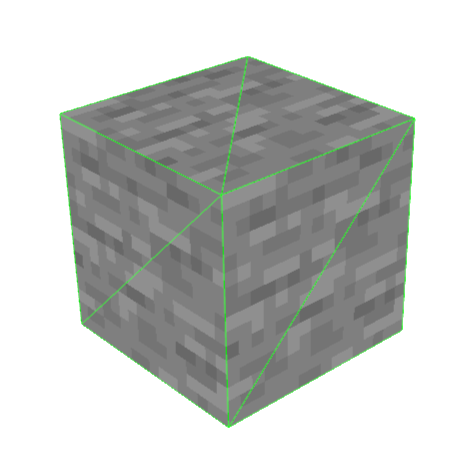
\includegraphics[width=0.8\textwidth]{../assets/single_voxel.png}
		\end{center}
	\end{minipage}\hfill
\end{figure}

\goodbreak

Ein Quadrat wird aus $2$ Dreiecken zusammengesetzt
und ein Würfel hat $6$ Seiten. Somit besteht ein Würfel
aus $12$ Dreiecken. Wenn der Spieler nur $100$ Voxels
weit sehen könnte, wäre der Durchmesser $200$ Voxels
und somit das gesamte Volumen, das angezeigt werden
muss $200^3 = 8.000.000$ Voxels groß, also
$12 \cdot 200^3 = 96.000.000$ Dreiecke.

Wir sehen also, dass schon bei einer sehr kleinen
Sichtweite sehr viele Dreiecke erstellt werden.
Diese Hausarbeit beschäftigt sich deswegen mit der
Optimierung, die Anzahl der Dreiecke so weit wie
möglich zu reduzieren.

Die meisten Optimierungen in dieser Hausarbeit
kommen von den Quellen \cite{yt_bin_greedy_mesher}
und \cite{gh_bin_greedy_mesher}, und wurden dann
noch ausgeweitet, damit sie auch für
Voxels mit Texturen funktionieren.
 }

{ \newcommand{\minipagespace}[1]{
	\begin{minipage}[c]{#1\textwidth}
		\ 
	\end{minipage}
}

\section{Culling}

Der erste Weg eine Voxel Engine zu optimieren wird
offensichtlich, wenn man einen Würfel aus $8$
Voxels betrachtet. Dabei beobachten wir, dass
die Hälfte der Seiten der Voxels nach innen schauen
und somit nicht sichtbar sind. Wenn man die
Seitenlänge dieses Würfels verdoppelt, multipliziert
man die Oberfläche mit $4$ und das Volumen mit $8$.
Somit entstehen immer mehr Seiten, die nach innen
schauen, umso größer das Objekt ist. Also wird
dies bei großen Objekten dazu führen, dass die
meisten Seiten nicht sichtbar sind.

\begin{center}
\begin{figure}[ht]
	\minipagespace{0.04}
	\begin{minipage}[c]{0.4\textwidth}
		\begin{center}
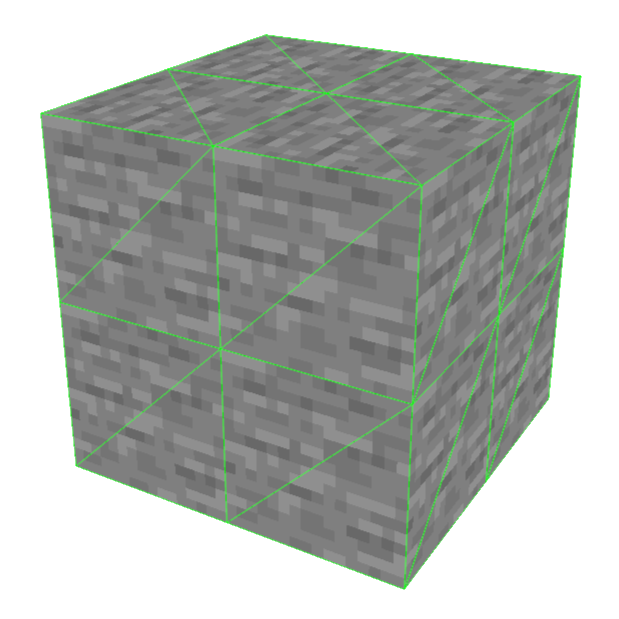
\includegraphics[width=1\textwidth]{../assets/culling/opaque_8_blocks.png}
		\end{center}
	\end{minipage}
	\minipagespace{0.09}
	\begin{minipage}[c]{0.4\textwidth}
		\begin{center}
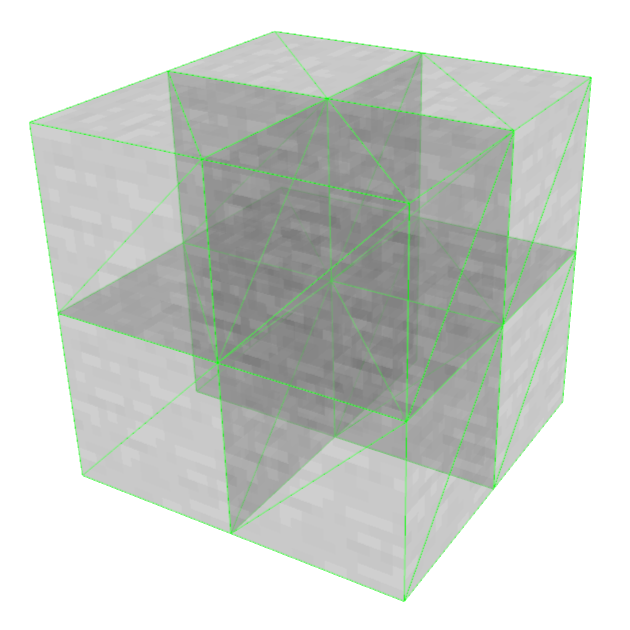
\includegraphics[width=1\textwidth]{../assets/culling/transparent_8_blocks.png}
		\end{center}
	\end{minipage}\hfill
\end{figure}
\end{center}

Mit \gqq{Culling} beschreibt man die Optimierung,
diese Seiten zu entfernen.

{ \subsection{Erste Implementation}

% TODO
 }

{ \subsection{Binäres Greedy Meshing}

Ich habe erst geplant, eine einfachere Implementation
von Greedy Meshing zu erstellen, bevor ich dies mit
einem binären Algorithmus mache, aber dadurch,
dass das Culling schon binär ist, ist die binäre
Greedy Meshing Implementation sogar einfacher als
eine andere.

Der Grundgedanke in dieser Implementation ist,
dass jedes Mal, wenn wir eine Seite betrachten,
wir versuchen diese erst in eine Richtung so weit
zu erweitern, bis keine Seite mehr da ist und dann
erweitern wir diesen ganzen Streifen in die andere
Richtung.
Während man das macht, entfernt man immer die
Bits in der Bitmaske, die gerade für diese Dreiecke
verwendet werden, damit sie nicht später für andere
Dreiecke wieder verwendet werden.

\begin{center}
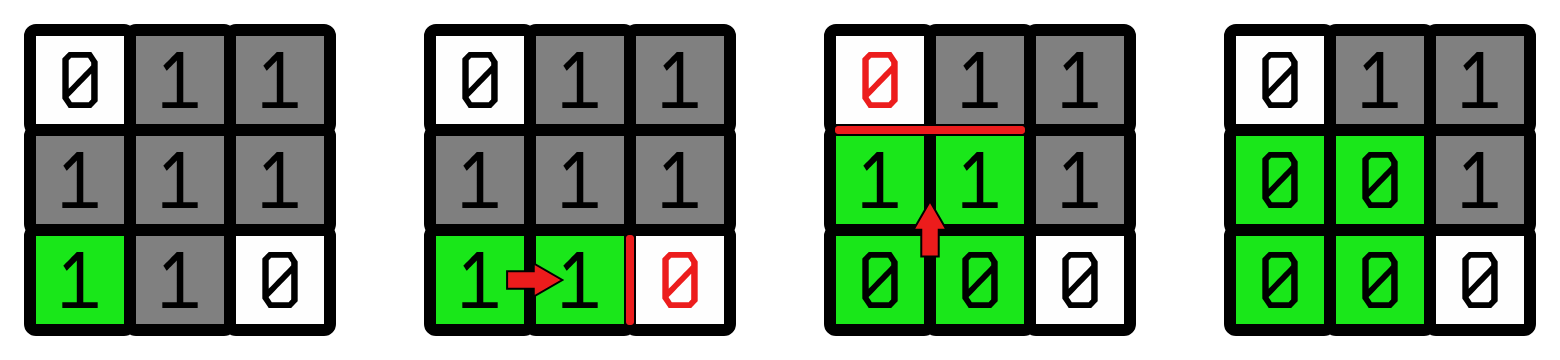
\includegraphics[width=0.95\textwidth]{../assets/greedy/grid_visualization.png}
\end{center}

Wenn wir eine Bitmaske haben, in der ein
32-Bit Integer eine Reihe von Seiten darstellt,
dann geht es sehr schnell, die Streifen zu erkennen,
da man mit den x86-Befehlen
\href{https://www.felixcloutier.com/x86/bsf}{BSF} \cite{bsf}
und
\href{https://www.felixcloutier.com/x86/bsr}{BSR} \cite{bsr}
die Anzahl von Nullen oder Einsen am Anfang oder
Ende eines 32-Bit Integers mit einem einzigen
Befehl berechnen kann.
Zudem kann man mit einem bitweisen ODER
überprüfen, ob der Streifen in die andere Richtung
erweitert werden kann, und man kann die Einträge
in der Bitmaske mit einem bitweisen UND entfernen.

\begin{lstlisting}[language=Rust]
let mut mask_copy = array[j];
let mut k = 0;
while mask_copy != 0 {
	let zeros = mask_copy.trailing_zeros();
	mask_copy >>= zeros;
	k += zeros;

	let ones = mask_copy.trailing_ones();
	mask_copy >>= ones;
	let from = k;
	k += ones;

	// Dieser gesamte Streifen als Bitmaske.
	// (Die wirkliche Implementation sieht etwas anders
	//  aus, da sich overflow von << komisch verhaelt)
	let strip_mask = ((1 << ones) - 1) << from;

	// Erweitere diesen Streifen in der Form eines Rechtecks
	// und entferne waehrenddessen 1en aus der Bitmaske.
	array[j] &= !strip_mask;
	let mut strip_expand = 0;
	for next_mask in &mut array[(j + 1)..] {
		if *next_mask & strip_mask == strip_mask {
			strip_expand += 1;
			*next_mask &= !strip_mask;
		} else {
			break;
		}
	}

	// erstelle ein Rechteck mit der richtigen Groesse...
}
\end{lstlisting}

Vielleicht ist Ihnen aber schon aufgefallen,
dass die Bitmaske, die wir für das Binäre Culling
verwendet haben, nicht in die richtige Richtung
ausgerichtet ist.
Dabei ist nämlich ein Integer eine Reihe von Voxels,
die sich gegenseitig verdecken können, während wir
hier eine Reihe von Voxels
(oder genauer: sichtbare Seiten)
brauchen, die nebeneinander liegen.
Deswegen müssen wir aus der Culling Bitmaske
eine neue Bitmaske konstruieren:

\begin{lstlisting}[language=Rust]
let culled_blocks_mask = // maske von Binaeres Culling
let mut greedy_mask = Box::<FaceMap<ChunkArray2D<u32>>>::default();
for (face, array2d) in culled_blocks_mask.iter_face() {
	for (i, array) in array2d.iter().enumerate() {
		for (j, mask) in array.iter().enumerate() {
			let mut mask = *mask;
			let mut k = 0;
			while mask != 0 {
				let zeros = mask.trailing_zeros();
				mask = (mask >> zeros) & !1;
				k += zeros;
				greedy_mask[face][k as usize][i] |= 1 << j;

				// Da horizontale Streifen von Voxels haeufiger
				// vorkommen als vertikale Streifen, mache ich,
				// dass die Bitmasken in den x- und z-Achsen
				// beide horizontal ausgerichtet sind.
				// Deswegen wird in der wirklichen Implementation
				// fuer die z-Achse `i` und `j` getauscht.
			}
		}
	}
}
greedy_mask
\end{lstlisting}

Wenn wir nun diese Bitmaske haben, können wir mit dem
oben genannten Algorithmus die Seiten zu größeren
Seiten kombinieren.
Wenn wir also diese Information benutzen,
um die Dreiecke größer zu machen, sind wir
schon mit dem Greedy Meshing fertig!

\vspace{0.5cm}

% Greedy Meshing 1 stats from: bench 11
\benchgraph{4}{0.25}{
	algo                   & blue       & red       \\
	Erste Implementation   & 12.834184  & 0.672563  \\
	Binäres Culling 1      &  2.883930  & 5.155590  \\
	Binäres Culling 2      &  8.524388  & 0.448866  \\
	Greedy Meshing 1       &  5.641821  & 0.425993  \\
}

Mit diesem Algorithmus erhalten wir sogar eine bessere
Performance, da wir weniger Dreiecke konstruieren
müssen.
Zudem ist die Anzahl von Dreiecken in einer
typischen Spielwelt jetzt von
1.857.984 Ecken und 928.992 Dreiecken
runter auf 809.484 Ecken und 404.742 Dreiecken
gesunken.
Somit haben wir etwa 2,3-mal weniger Dreiecke.

\vspace{0.7cm}

{
	\setlength{\parindent}{0pt}
	... eigentlich sind wir aber noch nicht ganz fertig!\\
	Wir haben noch ein Problem übersehen.
}
 }
 }

\pagebreak

{ \section{Greedy Meshing}

Nun kommen wir zum zweiten Weg eine Voxel Engine
zu optimieren:

\begin{center}
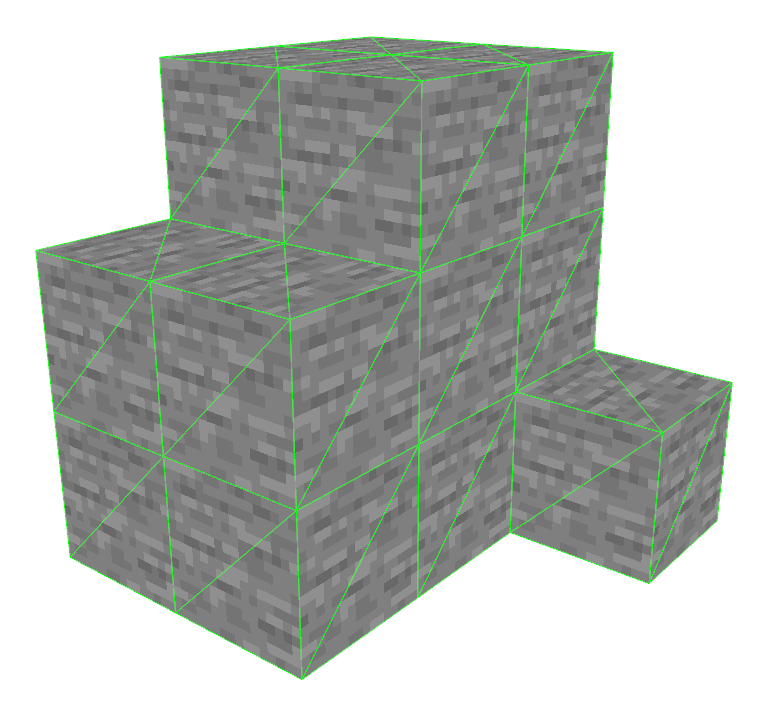
\includegraphics[width=0.4\textwidth]{../assets/greedy/stone_simple.png}
\end{center}

In der Grafik oben gibt es viele flache Flächen,
die aus unnötig vielen Dreiecken aufgebaut sind.
Wir könnten es wie folgt in Dreiecke einteilen,
um die Anzahl zu reduzieren:

\begin{center}
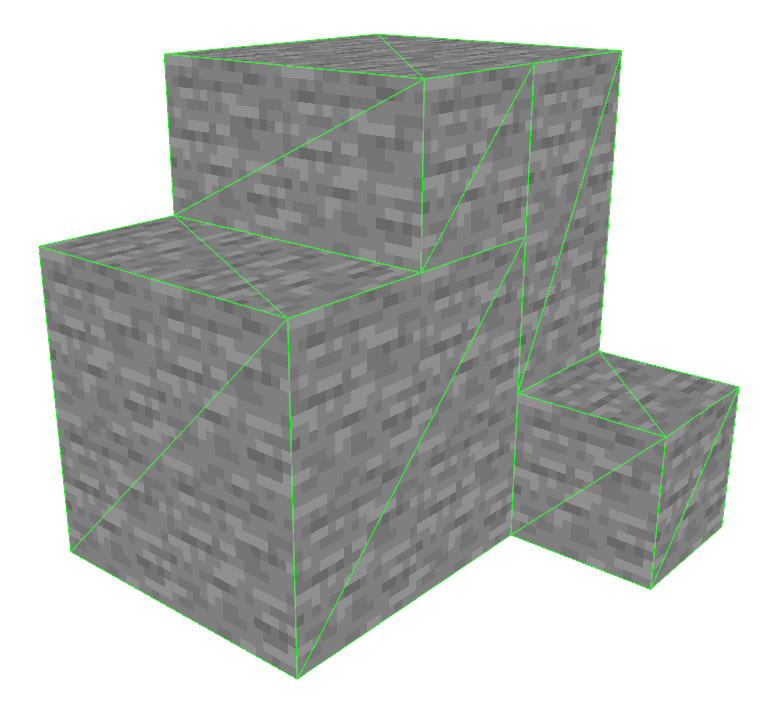
\includegraphics[width=0.4\textwidth]{../assets/greedy/stone_greedy.png}
\end{center}

Somit werden zum Beispiel nur 2 Dreiecke verwendet,
um eine 2x2 Fläche von Voxels zu bilden,
anstatt 8 Dreiecke.

Diese Optimierung wird \gqq{Greedy Meshing} genannt.

{ \subsection{Binäres Greedy Meshing}

Ich habe erst geplant, eine einfachere Implementation
von Greedy Meshing zu erstellen, bevor ich dies mit
einem binären Algorithmus mache, aber dadurch,
dass das Culling schon binär ist, ist die binäre
Greedy Meshing Implementation sogar einfacher als
eine andere.

Der Grundgedanke in dieser Implementation ist,
dass jedes Mal, wenn wir eine Seite betrachten,
wir versuchen diese erst in eine Richtung so weit
zu erweitern, bis keine Seite mehr da ist und dann
erweitern wir diesen ganzen Streifen in die andere
Richtung.
Während man das macht, entfernt man immer die
Bits in der Bitmaske, die gerade für diese Dreiecke
verwendet werden, damit sie nicht später für andere
Dreiecke wieder verwendet werden.

\begin{center}
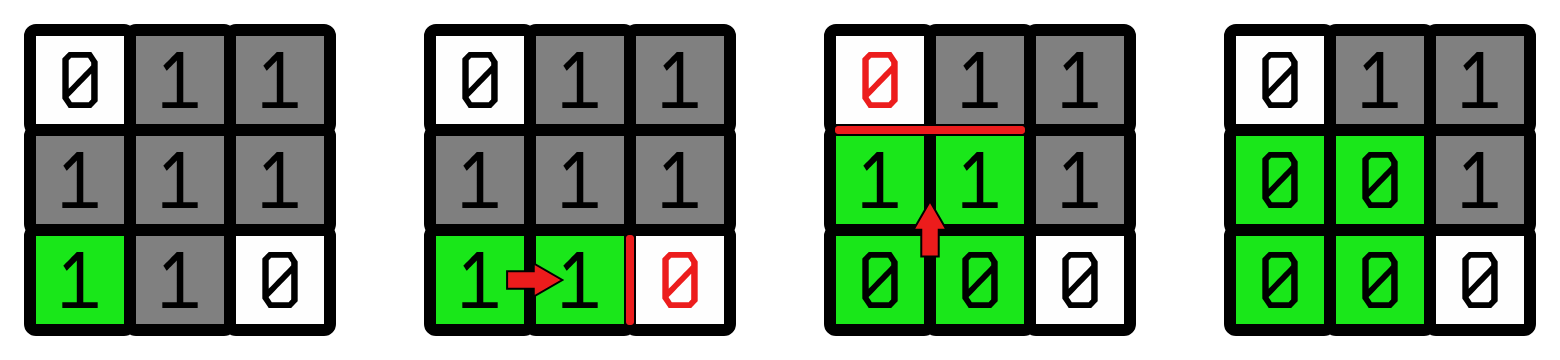
\includegraphics[width=0.95\textwidth]{../assets/greedy/grid_visualization.png}
\end{center}

Wenn wir eine Bitmaske haben, in der ein
32-Bit Integer eine Reihe von Seiten darstellt,
dann geht es sehr schnell, die Streifen zu erkennen,
da man mit den x86-Befehlen
\href{https://www.felixcloutier.com/x86/bsf}{BSF} \cite{bsf}
und
\href{https://www.felixcloutier.com/x86/bsr}{BSR} \cite{bsr}
die Anzahl von Nullen oder Einsen am Anfang oder
Ende eines 32-Bit Integers mit einem einzigen
Befehl berechnen kann.
Zudem kann man mit einem bitweisen ODER
überprüfen, ob der Streifen in die andere Richtung
erweitert werden kann, und man kann die Einträge
in der Bitmaske mit einem bitweisen UND entfernen.

\begin{lstlisting}[language=Rust]
let mut mask_copy = array[j];
let mut k = 0;
while mask_copy != 0 {
	let zeros = mask_copy.trailing_zeros();
	mask_copy >>= zeros;
	k += zeros;

	let ones = mask_copy.trailing_ones();
	mask_copy >>= ones;
	let from = k;
	k += ones;

	// Dieser gesamte Streifen als Bitmaske.
	// (Die wirkliche Implementation sieht etwas anders
	//  aus, da sich overflow von << komisch verhaelt)
	let strip_mask = ((1 << ones) - 1) << from;

	// Erweitere diesen Streifen in der Form eines Rechtecks
	// und entferne waehrenddessen 1en aus der Bitmaske.
	array[j] &= !strip_mask;
	let mut strip_expand = 0;
	for next_mask in &mut array[(j + 1)..] {
		if *next_mask & strip_mask == strip_mask {
			strip_expand += 1;
			*next_mask &= !strip_mask;
		} else {
			break;
		}
	}

	// erstelle ein Rechteck mit der richtigen Groesse...
}
\end{lstlisting}

Vielleicht ist Ihnen aber schon aufgefallen,
dass die Bitmaske, die wir für das Binäre Culling
verwendet haben, nicht in die richtige Richtung
ausgerichtet ist.
Dabei ist nämlich ein Integer eine Reihe von Voxels,
die sich gegenseitig verdecken können, während wir
hier eine Reihe von Voxels
(oder genauer: sichtbare Seiten)
brauchen, die nebeneinander liegen.
Deswegen müssen wir aus der Culling Bitmaske
eine neue Bitmaske konstruieren:

\begin{lstlisting}[language=Rust]
let culled_blocks_mask = // maske von Binaeres Culling
let mut greedy_mask = Box::<FaceMap<ChunkArray2D<u32>>>::default();
for (face, array2d) in culled_blocks_mask.iter_face() {
	for (i, array) in array2d.iter().enumerate() {
		for (j, mask) in array.iter().enumerate() {
			let mut mask = *mask;
			let mut k = 0;
			while mask != 0 {
				let zeros = mask.trailing_zeros();
				mask = (mask >> zeros) & !1;
				k += zeros;
				greedy_mask[face][k as usize][i] |= 1 << j;

				// Da horizontale Streifen von Voxels haeufiger
				// vorkommen als vertikale Streifen, mache ich,
				// dass die Bitmasken in den x- und z-Achsen
				// beide horizontal ausgerichtet sind.
				// Deswegen wird in der wirklichen Implementation
				// fuer die z-Achse `i` und `j` getauscht.
			}
		}
	}
}
greedy_mask
\end{lstlisting}

Wenn wir nun diese Bitmaske haben, können wir mit dem
oben genannten Algorithmus die Seiten zu größeren
Seiten kombinieren.
Wenn wir also diese Information benutzen,
um die Dreiecke größer zu machen, sind wir
schon mit dem Greedy Meshing fertig!

\vspace{0.5cm}

% Greedy Meshing 1 stats from: bench 11
\benchgraph{4}{0.25}{
	algo                   & blue       & red       \\
	Erste Implementation   & 12.834184  & 0.672563  \\
	Binäres Culling 1      &  2.883930  & 5.155590  \\
	Binäres Culling 2      &  8.524388  & 0.448866  \\
	Greedy Meshing 1       &  5.641821  & 0.425993  \\
}

Mit diesem Algorithmus erhalten wir sogar eine bessere
Performance, da wir weniger Dreiecke konstruieren
müssen.
Zudem ist die Anzahl von Dreiecken in einer
typischen Spielwelt jetzt von
1.857.984 Ecken und 928.992 Dreiecken
runter auf 809.484 Ecken und 404.742 Dreiecken
gesunken.
Somit haben wir etwa 2,3-mal weniger Dreiecke.

\vspace{0.7cm}

{
	\setlength{\parindent}{0pt}
	... eigentlich sind wir aber noch nicht ganz fertig!\\
	Wir haben noch ein Problem übersehen.
}
 }

{ \subsection{Korrektur der Texturen}

% TODO

% Greedy Meshing 2 stats from: bench 13
\benchgraph{5}{0.2}{
	algo                   & blue       & red       \\
	Erste Implementation   & 12.834184  & 0.672563  \\
	Binäres Culling 1      &  2.883930  & 5.155590  \\
	Binäres Culling 2      &  8.524388  & 0.448866  \\
	Greedy Meshing 1       &  5.641821  & 0.425993  \\
	Greedy Meshing 2       &  7.092519  & 0.317280  \\
}
 }
 }

\pagebreak

{ \section{Fazit}

% TODO
 }

{ \section{Quellen / Literaturverzeichnis}


% remove the extra title inserted by thebibliography
\renewcommand{\section}[2]{}

\begin{thebibliography}{9}

\setlength{\itemindent}{0.5cm}

\bibitem{yt_bin_greedy_mesher}
\url{https://youtu.be/qnGoGq7DWMc?si=Ke8vgcHWcgCdMGka}

\bibitem{gh_bin_greedy_mesher}
\url{https://github.com/TanTanDev/binary_greedy_mesher_demo}

\bibitem{wiki_volume}
\url{https://de.wikipedia.org/wiki/Volumengrafik}

\bibitem{wiki_poly}
\url{https://de.wikipedia.org/wiki/Polygonnetz}

\bibitem{wiki_thread}
\url{https://de.wikipedia.org/wiki/Thread_(Informatik)}

\bibitem{wiki_wettlauf}
\url{https://de.wikipedia.org/wiki/Wettlaufsituation}

\bibitem{nomicon_races}
\url{https://doc.rust-lang.org/nomicon/races.html}

\bibitem{bevy_systems}
\url{https://bevy-cheatbook.github.io/programming/systems.html}

\end{thebibliography}


\vspace{0.2cm}

\setlength{\parindent}{0pt}

Der Quellcode für dieses \LaTeX\ Dokument: \\
\url{https://github.com/BlueSheep3/MINT-Hausarbeit}.

\vspace{0.2cm}

Meine Implementation dieser Optimierungen: \\
\url{https://github.com/BlueSheep3/voxel_game}.
 }

\vspace*{\fill}

{
\setlength{\parindent}{0pt}

Hiermit versichere ich, dass ich die vorliegende
Hausarbeit selbständig verfasst und keine anderen
als die angegebenen Hilfsmittel benutzt habe.


\includegraphics[width=0.4\textwidth]{../assets/signature.png}

Marburg, \today
}

\vspace{1cm}


\end{document}
